\documentclass[a4paper, 8pt]{extarticle}

\usepackage[greek,spanish,es-tabla,es-nodecimaldot,es-noindentfirst]{babel}

\usepackage[a4paper, lmargin=0.2cm,rmargin=0.2cm,tmargin=1cm,bmargin=1cm, landscape]{geometry}
\usepackage{multicol}
\usepackage{amsmath}
\usepackage{mathtools}
\usepackage{cancel}
\usepackage{siunitx}
\usepackage{physics}
\usepackage{enumitem}
\usepackage{circuitikz}
\usepackage{graphicx}
\usepackage{xcolor}
\usepackage{xspace}

% For Excel2LaTeX tables
\usepackage{colortbl}
\usepackage{booktabs}

\AtBeginDocument{\RenewCommandCopy\qty\SI}
\usepackage{esvect}
\renewcommand{\vec}[1]{\vv{{#1}}}
\renewcommand{\grad}{\nabla}

\usepackage{lmodern}
\renewcommand{\familydefault}{\sfdefault}
\renewcommand{\rmdefault}{\sfdefault}

\renewcommand{\sin}{\sen}

\usepackage{titlesec}
\titleformat{\section}
  {\normalfont\Large\bfseries}{\thesection}{1em}{}[{\titlerule[0.8pt]}]

\titlespacing*{\section}{0pt}{4pt plus 0pt minus 0pt}{5pt plus 2pt minus 2pt}
\titlespacing*{\subsection}{0pt}{4pt plus 0pt minus 0pt}{3pt plus 2pt minus 2pt}
\titlespacing*{\subsubsection}{0pt}{4pt plus 0pt minus 0pt}{3pt plus 2pt minus 2pt}

\allowdisplaybreaks
\setcounter{secnumdepth}{-1}
\setcounter{tocdepth}{-1}

%%% INICIO DEL DOCUMENTO %%%
\begin{document}

\setlength{\parskip}{0pt}
\setlength{\parindent}{0pt}
\setlist{nosep}
\setlength{\abovedisplayskip}{2pt}
\setlength{\belowdisplayskip}{2pt}
\setlength{\abovedisplayshortskip}{0pt}
\setlength{\belowdisplayshortskip}{0pt}


\pagestyle{empty}
\renewcommand{\arraystretch}{1.5}

\begin{multicols}{3}
  \section{T3. Micrófonos}
  \subsection{Características de los micrófonos}
  \subsubsection{Sensibilidad}
  La sensibilidad de un micrófono es la \textbf{relación entre la tensión eléctrica generada y la presión acústica incidente} (en circuito abierto, campo libre, a \qty{1}{\kilo\hertz}).
  \begin{align*}
    S & = \frac{E_{\text{c.a.}}}{p} \ \left[ \unit{\volt \per \pascal }  \right]                                                                            \\
      & = 20 \log \left( \frac{\abs{S}}{\qty{1}{\volt \per \pascal  } } \right) \ \left[ \unit{\decibel} \text{ re. } \qty{1}{\volt \per \pascal }  \right]
  \end{align*}
  La sensibilidad de referencia es la sensibilidad medida en el eje del micrófono.
  \[ S_0 = S \left( \theta = \ang{0} \right) \]
  \subsubsection{Respuesta en frecuencia}
  La respuesta en frecuencia de un micrófono es la \textbf{variación de la sensibilidad con la frecuencia} $\left[ S = S(f) \right]$. Se suele representar la respuesta relativa con respecto a la sensibilidad de referencia en decibelios.
  \[ S(f) - S_0 = 20 \log \left( \frac{\abs{S(f)}}{\abs{S_0}} \right) \ \unit{\dB} \]
  La presencia del micrófono afecta a su respuesta. La respuesta del diafragma en alta frecuencia aumenta la presión frente a la cápsula.

  \color{red}\xspace
  \subsubsection{Distorsión lineal}
  \begin{itemize}
    \item \textbf{Coloraciones.} La respuesta en frecuencia no es plana.
    \item \textbf{Vibraciones parciales del diafragma.} Debidas a modos propios. Los micros de condensador no tienen este problema.
    \item \textbf{Resonancias mecánicas o acústicas.} Sobre todo en micros dinámicos.
    \item \textbf{Ancho de banda limitado por componentes eléctricos.}
    \item \textbf{Distorsión de fase.}
  \end{itemize}
  \subsubsection{Distorsión no lineal}
  \begin{itemize}
    \item \textbf{Saturación.} Sobrecarga de presión. Si saturan fácilmente se llaman micros \textit{blandos}. Si no, \textit{duros}.
    \item \textbf{Pop.} Chorros de aire (no sonido). Suele ser por fonemas ``explosivos''.
  \end{itemize}
  \color{black}\xspace
  \subsubsection{Directividad}
  Generalmente, su supone simetría cilíndrica de los micrófonos, por lo que la directividad no depende del plano azimutal $\varphi$.
  \begin{align*}
    D(\theta, \varphi )          & \equiv \text{Directividad}                                         \\
    Q(\theta, \varphi )          & \equiv \text{Factor de directividad}                               \\
    Q _{\textnormal{ax}}         & \equiv \text{Factor de directividad axial (en el eje)}             \\
    \text{DI}                    & \equiv \text{Índice de directividad}                               \\
    \text{DI} _{\textnormal{ax}} & \equiv \text{Índice de directividad axial (en el eje)}             \\
    \text{REE}                   & \equiv \text{Eficiencia de energía aleatoria}                      \\
    \text{DSF}                   & \equiv \text{Factor de distancia}                                  \\
    E_d                          & \equiv \text{Tensión directa}                                      \\
    E_r                          & \equiv \text{Tensión reverberante}                                 \\
    E_{ro}                       & \equiv \text{Tensión reverberante del equivalente omnidireccional} \\
  \end{align*}.

  Si especifican que se ha medido en cámara anecoica, entonces se refiere a que $E_{\text{c.a.}}$ es también el valor de $E_d$.
  \begin{align*}
    p_d (r) & = \frac{p (\qty{1}{\metre } )}{r} \qquad E_d = p_d (r) S                                                                  \\
    E_r     & = \frac{p_r S_0}{\sqrt{Q _{\textnormal{ax}}}} \qquad \langle E_d^2(\theta, \varphi) \rangle = E_r^2 \qquad E_{ro} = p_r S
  \end{align*}
  La distancia crítica $r_c$ es la distancia a partir de la cual la presión reverberante es igual a la directa. En ella la tensión total y presión total serán:
  \begin{align*}
    E_{t}           & = \sqrt{E_r ^2 + E_d ^2}                   & p_0 = p_r = p_d = \frac{p_{t}}{\sqrt{2}} \\
    E_{t} (\theta ) & = p_0 S_0 \sqrt{D^2(\theta ) + \text{REE}}
  \end{align*}
  Recordamos que es suma no coherente por ser campo difuso.
  \begin{align*}
    D( \theta)          & = \frac{S(\theta)}{S_0 } \qquad Q(\theta, \varphi ) = Q _{\textnormal{ax}} D^2                                                    (\theta, \varphi )                                                                              \\
    Q(\theta, \varphi ) & = \frac{S^2(\theta, \varphi )}{\langle S^2(\theta, \varphi) \rangle} = \frac{S^2(\theta, \varphi )}{\frac{1}{4\pi} \int_{\varphi = 0}^{2\pi} \int_{\theta = 0}^{\pi} S^2(\theta, \varphi) \sin (\theta ) \dd \theta \dd \varphi } \\
    Q_{\textnormal{ax}} & = Q(\theta = \ang{0}) = \frac{2}{\int_{\theta = 0}^{\pi} D^2(\theta) \sin (\theta ) \dd \theta } \approx \frac{2}{\frac{\pi}{N} \sum _{i=1}^{N} D^2(\theta _i) \sin (\theta i)}                                                   \\
    Q_{\textnormal{ax}} & = \frac{E^2_{ro}} {E^2_r} \eval*{}_{\text{campo difuso}} \quad \text{DI} = 10 \log \left[ Q( \theta, \varphi) \right] \qquad \text{DI} _{\textnormal{ax}} = 10 \log \left( Q_{\textnormal{ax}} \right)                            \\
    \text{REE}          & = \frac{1}{Q_ {\textnormal{ax}}} \qquad \text{DSF} = \sqrt{Q_{\textnormal{ax}}}                                                                                                                                                   \\
  \end{align*}

  \textbf{Nota 1:} En la fórmula de $Q_{\textnormal{ax}}$ para $N$ valores, si nos dicen que supongamos simetría de revolución se usan los valores entre $\theta = \ang{0}$ y $\theta = \ang{180}$, sin incluir este último. Si da tiempo (y en entornos reales), se calculan tanto en el intervalo $[0, 180)$ como en $[180, 360)$ y se hace la media entre ambos $Q_{\textnormal{ax}}$ obtenidos.

  \textbf{Nota 2:} Si nos piden sacar la directividad sabiendo que es de familia cardioide y no dicen nada más, debemos suponer orden $n=1$.
  \subsubsection{Directividad de la familia cardiode}
  $A$ es el componente omnidireccional, $B$ el componente bidireccional y $n$ el orden de la directividad.

  \[\left\lbrace
    \begin{matrix*}[l]
      D (\theta ) = \left[ A + B \cos (\theta ) \right] \cos ^{n-1} (\theta )  \\
      A + B = 1
    \end{matrix*}\right.\]


  % Table generated by Excel2LaTeX from sheet 'Sheet1'
  \begin{center}
    \begin{tabular}{|c|c|l|}
      \hline
      \rowcolor[rgb]{ .663,  .816,  .557} A    & B    & \multicolumn{1}{c|}{Tipo} \\
      \hline
      \rowcolor[rgb]{ .886,  .937,  .855} 0.50 & 0.50 & Cardioide                 \\
      \hline
      \rowcolor[rgb]{ .886,  .937,  .855} 0.75 & 0.25 & Subcardioide              \\
      \hline
      \rowcolor[rgb]{ .886,  .937,  .855} 0.25 & 0.75 & Hipercardioide            \\
      \hline
    \end{tabular}
  \end{center}

  Si $n = 1$, el valor de $Q _{\textnormal{ax}}$ viene dado por la resolución de la integral de su definición, el resultado es este:

  \[ Q _{\textnormal{ax}} = \frac{3}{4B^2 - 6B + 3} \]

  \color{red}\xspace
  \subsubsection{Ruido eléctrico}

  \begin{itemize}
    \item \textbf{Ruido eléctrico.} Tensión de salida del micrófono cuando no recibe excitación acústica. Causado por:
          \begin{itemize}
            \item Agitación térmica de moléculas de aire o del diafragma.
            \item Agitación térmica electrónica, debi principalmente a resistencias altas.
          \end{itemize}
          \[ E_N = \sqrt{4kTR \Delta f} \ \left[ \unit{\volt }  \right]\]
          Donde $k$ es la constante de Boltzmann, $T$ la temperatura, $R$ la resistencia y $\Delta f$ el ancho de banda. Se suele expresar en \unit{\dB_{\text{SPL}}} y se denomina ``nivel de presión sonora equivalente al ruido'':
          \[ \text{ENL} = 20 \log \left( \frac{p_N}{p _{\textnormal{ref}}} \right)  = 20 \log \left( \frac{E_N}{p _{\textnormal{ref}}S_0} \right) \]
          Donde $p _{\textnormal{ref}} = \qty{20}{\micro\pascal }$. Para usar esta expresión, mencionar que se debería filtrar $E_N$ con un filtro de ponderación A.
    \item \textbf{Ruido por zumbido electromagnético (\textit{hum}).}
    \item \textbf{Ruido por viento.}
  \end{itemize}

  \subsubsection{Márgenes dinámicos}

  \begin{align*}
    \text{Margen dinámico}        & \qquad \text{DR} = \text{SPL}_{\text{máx}} - \text{ENL}                                    \\
    \text{Margen de sobrecarga}   & \qquad \text{HR} = \text{SPL}_{\text{máx}} - 94 \ (\text{viene de } p _{\textnormal{ref}}) \\
    \text{Relación señal a ruido} & \qquad \text{SNR} = \text{DR} - \text{HR} = 94 - \text{ENL}
  \end{align*}
  \color{black}\xspace
  \subsection{Tipos de micrófonos}
  \subsubsection{TAM: Micrófonos de presión}
  La cápsula está compuesta por un diafragma y un pequeño orificio de ecualización, que sirve para regular la presión interna. La vibración del diafragma es proporcional a la presión acústica externa ejercida sobre el diafragma.
  \begin{center}
    \includegraphics[width=0.8\linewidth]{Mic de presión.png}
  \end{center}
  Presentan un comportamiento omnidireccional, excepto a alta frecuencia debido a difracción cuando $\lambda >> D$, siendo $D$ la mayor dimensión del micrófono. Para $\theta = \pm \ang{90}$, la directividad disminuye ligeramente por falta de uniformidad. Para $\theta = \ang{180}$, la directividad disminuye ligeramente por la sombra que genera la cápsula.

  \subsubsection{TAM: Micrófonos de gradiente de presión}

  La presión en la cara interna del diafragma es aproximadamente igual que en la cara externa. La diferencia de caminos acústicos entre ambas caras es la que hace que no sean iguales. Por lo tanto existe un incremento muy pequeño de presión entre ambas caras, es decir, un diferencial. De ahí viene el término gradiente de presión.
  \vspace*{\fill}
  \begin{center}
    \includegraphics[width=0.4\linewidth]{Mic grad de presión.png}
  \end{center}

  El \textbf{efecto proximidad} sucede cuando $kx << 1$ e implica que para bajas frecuencias (o micro muy cerca de la fuente) las ondas presentan divergencia esférica. Es decir, acercar el micro a la fuente incrementará la tensión generada. Esto no sucede para agudos porque $kx >> 1$ y las ondas son planas (sin divergencia esférica).
  \includegraphics[width=\linewidth]{Gradiente de presión.png}

  \[ \left\lbrace
    \begin{matrix*}[l]
      \lambda >> \Delta L & \longrightarrow D (\theta ) = \cos (\theta )\\
      \lambda << \Delta L & \longrightarrow \abs{D (\theta )} = \abs{\sin \left( \frac{k \Delta L \cos (\theta)}{2} \right)}
    \end{matrix*} \right. \]

  Como el efecto proximidad sucede si $kx << 1$, entonces $f _{\textnormal{prox}} = \frac{c}{2 \pi x}$. Teniendo que $F$ es la fuerza ejercida sobre el diafragma, entonces:

  \begin{align*}
    F                      & = 2jp e^{- \frac{jk \Delta L \cos (\theta)}{2}} \sin \left( \frac{k \Delta L \cos (\theta)}{2} \right) S_d \\
    G _{\textnormal{prox}} & = \frac{F}{F _{\textnormal{ondas planas}}} = \frac{1 + jkx}{jkx}
  \end{align*}

  \subsubsection{TAM: Micrófonos combinados de presión/gradiente de presión}
  Son como los micrófonos de presión cambiando el orificio de ecualización por una abertura de mayor tamaño, conformando un sistema acústico. El principio de funcionamiento es el mismo que los micrófonos de gradiente de presión.
  \begin{align*}
     & \left( k \dd L << 1 \right) \equiv \left( \dd L << \lambda \right)                                                             \\
     & \left\lbrace
    \begin{matrix*}[l]
      k \dd L << 1 & \longrightarrow D (\theta ) = \frac{K + \cos (\theta)}{K + 1}                                                      \\
      k \dd L >> 1 & \longrightarrow \abs{D (\theta )} = \abs{\sin \left( \frac{k\Delta L \left[ \cos (\theta + K) \right]}{2} \right)}
    \end{matrix*} \right. \\
     & \left\lbrace
    \begin{matrix*}[l]
      K = 1 \ \rightarrow \text{ cardioide} \\
      K = \frac{1}{3} \ \rightarrow \text{ hipercardioide} \\
      K = 0 \ \rightarrow \text{ bidireccional} \\
      K > 1 \ \rightarrow \text{ subcardioide}
    \end{matrix*}
    \right.  \qquad  A = \frac{K}{K + 1} \qquad B = \frac{1}{K + 1}
  \end{align*}
  \[ F = 2jp e^{- \frac{jk \Delta L \cos (\theta)}{2}} \sin \left( \frac{k \Delta L \cos (\theta)}{2} \right) S_d \]

  \subsubsection{TME: Micrófonos de bobina móvil}
  \subsubsection{TME: Micrófonos de cinta}
  \subsubsection{TME: Micrófonos electrostáticos de condensador}
  \subsubsection{TME: Micrófonos electrostáticos de electret (o prepolarizados)}
  \subsubsection{TME: Micrófonos MEMS}
  \subsubsection{Especiales: Micrófonos de doble diafragma}
  \subsubsection{Especiales: Micrófonos superdirectivos}
  \subsubsection{Especiales: Micrófonos lavalier}
  \subsubsection{Especiales: Micrófonos de superficie o de zona de presión}
  \subsubsection{Especiales: Micrófonos inalámbricos}
  \subsubsection{Técnica M/S}

  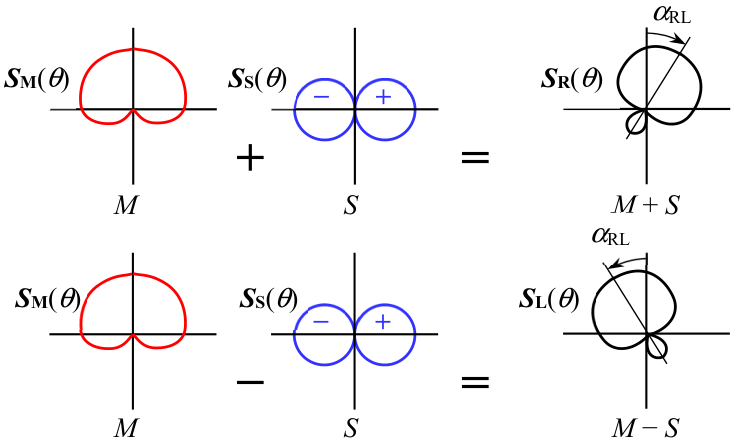
\includegraphics[width=0.8\linewidth]{Micros MS.png}
  Un micro cardioide y otro bidireccional. El ángulo $\alpha $ (que en las figuras aparece como $\alpha _{RL}$) representa el ángulo del cardioide producido con respecto al eje del conjunto de micrófonos.
  \begin{align*}
    S_R (\theta )               & = S_M (\theta ) + S_S (\theta )                                                \\
    S_L (\theta )               & = S_M (\theta ) - S_S (\theta )                                                \\
    S_0                         & = S_{M0} \left( A_M + \frac{B_M}{\cos (\alpha )} \right)                       \\
    \tan \left( \alpha  \right) & = \frac{S_{S0}}{B_M S_{M0}}                                                    \\
    B                           & = \frac{B_M}{A_M \cos (\alpha ) + B_M}                                         \\
    S_{M0}                      & = 2 S_0 \left[A_M + B_M \cos (\alpha ) \right]                                 \\
    S_{S0}                      & = 2 S_0 B \sin (\alpha )                                                       \\
    S_M ( \theta )              & = S_R ( \theta ) + S_L ( \theta ) = S_{M0} \left[ A + B \cos (\theta ) \right] \\
    S_S ( \theta )              & = S_R ( \theta ) - S_L ( \theta ) = S_{S0} \sen (\theta )
  \end{align*}

  \subsubsection{Técnica XY}
  Micros coincidentes, con ángulo de separación $\alpha$.
  \begin{align*}
    S_R (\theta )  & = S(\theta - \alpha )             \\
    S_L (\theta )  & = S(\theta + \alpha  )            \\
    S_M ( \theta ) & = S_R ( \theta ) + S_L ( \theta ) \\
    S_S ( \theta ) & = S_R ( \theta ) - S_L ( \theta )
  \end{align*}


  \subsection{Conexión eléctrica de los micrófonos}
  \subsubsection{Impedancias características}
  \subsubsection{Efecto del cable en la banda de frecuencias transmitida}
  \subsubsection{Línea microfónica balanceada}
  \subsubsection{Alimentación de micrófonos electrostáticos}
  \subsubsection{Adaptadores, conversores y distribuidores microfónicos}

  \newpage
  \section{T4. Sistemas de Refuerzo Sonoro}

  \subsection{Niveles acústicos}
  \subsubsection{Niveles de presión directo y reverberante}
  \subsubsection{Constante acústica de la sala}
  \subsubsection{Modificadores acústicos}
  \subsubsection{Distancia crítica}
  \subsubsection{Campo semirreverberante}
  \subsubsection{Niveles debidos a varias fuentes}
  \subsubsection{Potencia acústica}

  \subsection{Respuesta temporal}
  \subsubsection{Molestia por ecos}
  \subsubsection{Efecto precedencia}
  \subsubsection{Respuesta temporal mediante simulación}
  \subsubsection{Auralización}

  \subsection{Inteligibilidad}
  \subsubsection{Índice de inteligibilidad del habla}
  \subsubsection{Pérdida de articulación de consonantes}
  \subsubsection{Índice de transmisión del habla}

  \subsection{Configuraciones de altavoces}
  \subsubsection{Sistema centralizado con un altavoz o un cluster}
  \subsubsection{Clusters y arrays de altavoces}
  \subsubsection{Sistema distribuidos de altavoces}

  \subsection{Realimentación acústica}
  \subsubsection{Modelo}
  \subsubsection{Realimentación por un solo camino y en campo libre}
  \subsubsection{Realimentación cuando existe reverberación}
  \subsubsection{Condición de oscilación según los niveles acústicos en los micrófonos}
  \subsubsection{Respuesta temporal de la realimentación}
  \subsubsection{Control de la realimentación acústica}

  \subsection{Ganancia acústica}
  \subsubsection{Distancia acústica equivalente}
  \subsubsection{Ganancia acústica necesaria y ganancia acústica potencial}
  \subsubsection{Uso de la ganancia acústica para el diseño de un sistema de refuerzo sonoro}
  \subsection{Amplificación}
  \subsubsection{Amplificación de baja impedancia}
  \subsubsection{Amplificación de alta impedancia, líneas de tensión constante}
  \subsubsection{Conexión de amplificadores}
  \subsubsection{Clases de amplificación}
  \subsubsection{Fuentes de alimentación}

\end{multicols}

\end{document}
